\section{Results}
\subsubsection{Quantitative Results}
We evaluate Q-learning Concatenated (QLCAT), Q-learning (QL), model-based RL
(MBRL) and Floyd-Warshall Reinforcement Learning (FWRL) on two metrics in two
different environments. The two metrics we use are Distance inefficiency and
average reward per episode. The baselines and metrics are explained in the
experiment section (\ref{sec:experiments}). The results are shown in
Figure~\ref{fig:ql-fw-grid-world-results}-\ref{fig:ql-fw-windy-world-rewards} 
We find that FWRL consistently achieves higher rewards, and lower distance
inefficiency than the baselines. The reward curves also show that FWRL learns to
find the higher reward much faster than the baselines, demonstrating higher
sample efficiency.

\begin{figure}%
  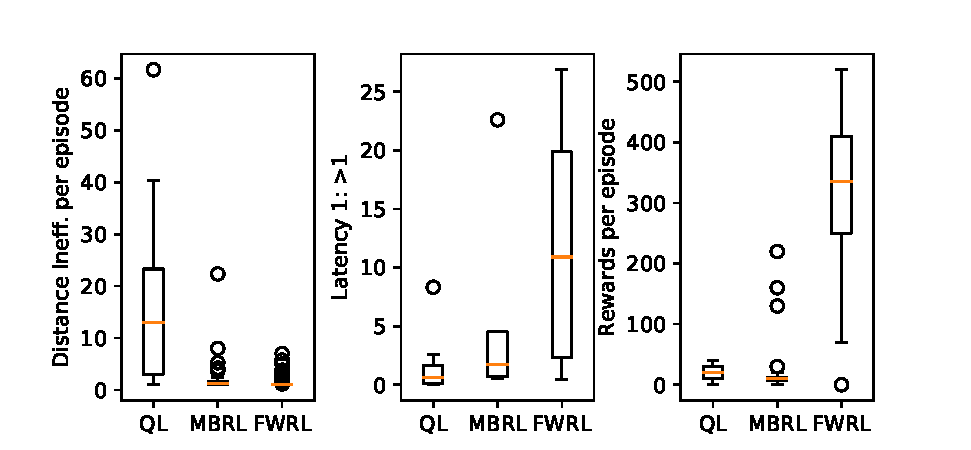
\includegraphics[width=\columnwidth]{./media/metrics-grid-world.pdf}{a}
  \caption{Results on grid world. FWRL beats other baselines
    consistently. Lower is better for Distance-Inefficiency. Higher
    is better for reward per episode. }
  \label{fig:ql-fw-grid-world-results}%
\end{figure}

\begin{figure}
  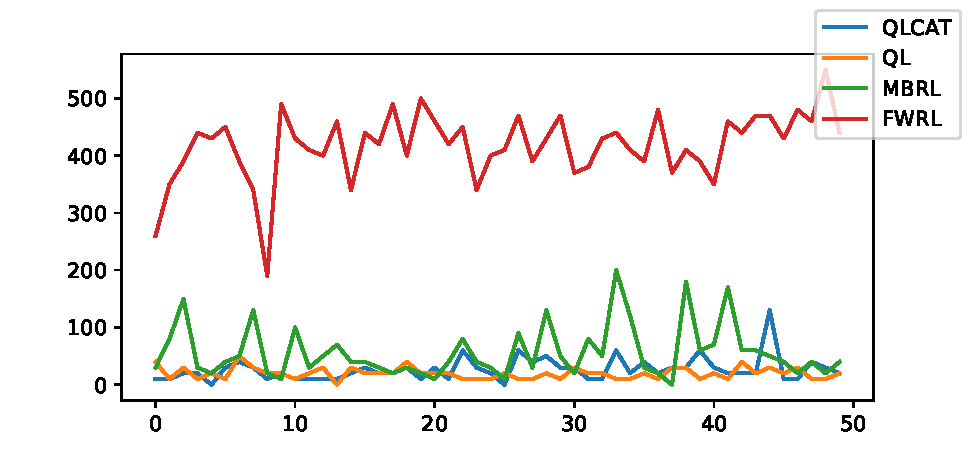
\includegraphics[width=\columnwidth]{./media/rewards-metrics-grid-world.pdf}{b}
  \caption{Reward curves on grid world. FWRL reward climbs much
    faster than all other baselines showcasing the improved \emph{sample
      efficiency} of the algorithm.}
  \label{fig:ql-fw-grid-world-reward-curves}%
\end{figure}

\begin{figure}
  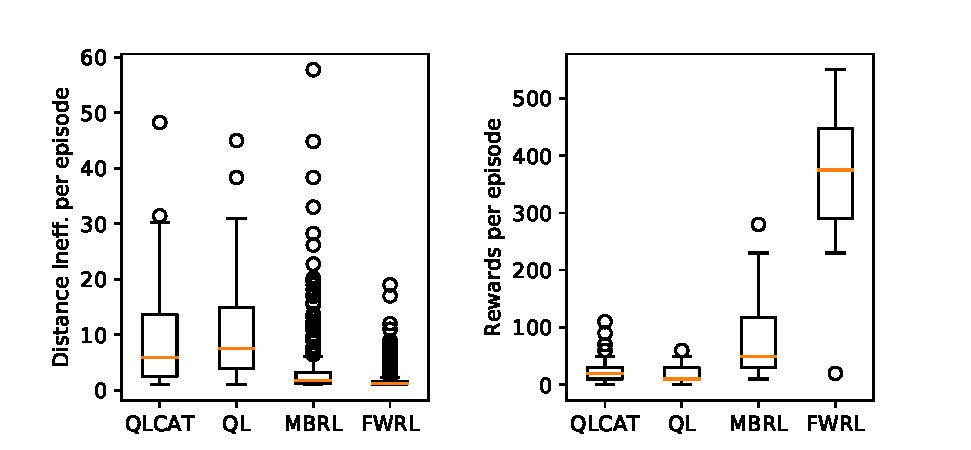
\includegraphics[width=\columnwidth]{./media/metrics-windy-world.pdf}
  \caption{Results on windy world. FWRL beats other baselines
    consistently. Lower is better for Distance-Inefficiency. Higher
    is better for reward per episode. }
  \label{fig:ql-fw-windy-world-results}%
\end{figure}

\begin{figure}
  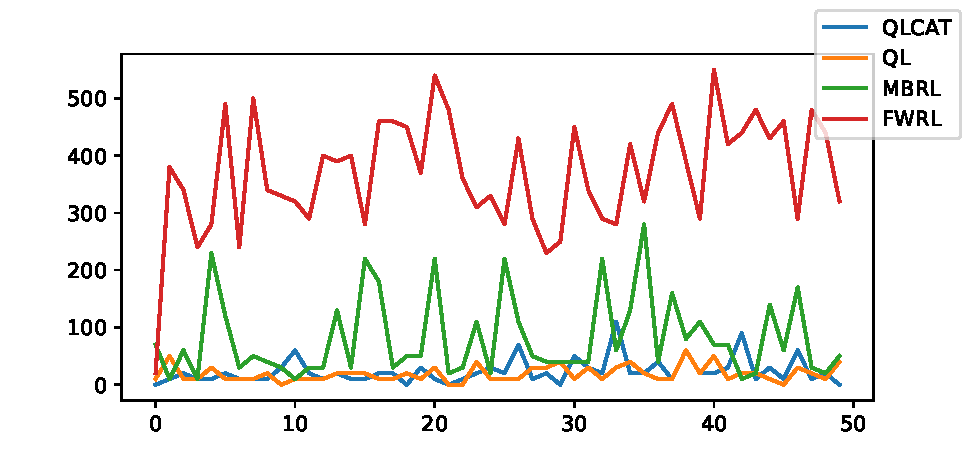
\includegraphics[width=\columnwidth]{./media/rewards-metrics-windy-world.pdf}
  \caption{Reward curves on windy world. FWRL reward climbs much
    faster than all other baselines showcasing the improved \emph{sample
      efficiency} of the algorithm.}
  \label{fig:ql-fw-windy-world-reward-curves}%
\end{figure}


\subsubsection{Qualitative Results}
To demonstrate the claim made in Fig~\ref{fig:visual-abstract}, we train QLCAT
and FWRL for two episodes each with start and goal locations such that the path
meets in the center. Unlike the quantitative section, in this experiment the
episode ends when the agent reaches the goal.
After two episodes of training, in which both FWRL (Floyd-Warshall RL) and QLCAT
(Q-Learning with goal concatenated to the state) reach the desired
goals via exploration, we put the algorithms to test.
For the test episode, the goal is chosen from first training episode but start
location is chosen from second training episode.
During the test episode,
we turn off $\epsilon$-greedy exploration and follow the learned policy
greedily.

We find that QLCAT decides to repeat the action that pushes it into the wall,
therefore is unable to move. However, FWRL reaches the goal using the shortest
path. The trajectories and value functions are visualized in Figure~\ref{fig:qualitative-results}.

\begin{figure}
  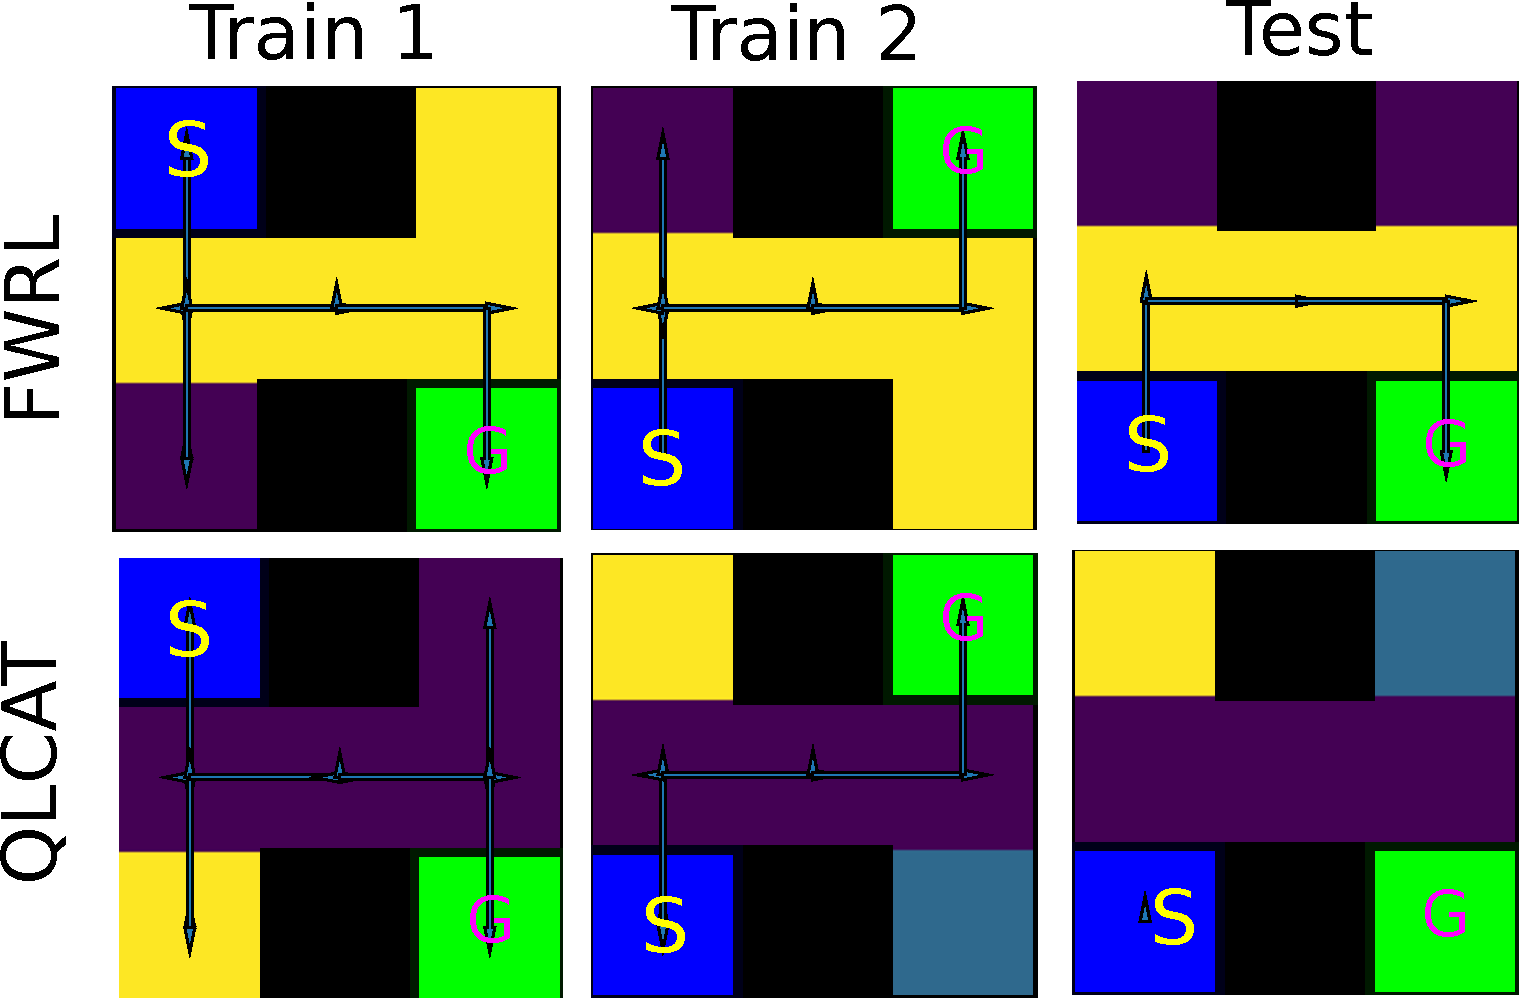
\includegraphics[width=\columnwidth]{./media/qualitative-results.pdf}
  \caption{Qualitative results: Visualization of value-function in H-Maze. Green
box with G represents goal location, Blue box with S represents start location.
The obstacles are shown black. The trajectories are shown by arrows. The color
of remaining boxes show the expected value of each state computed by the
corresponding algorithm. Each row different algorithm, while columns show
different episodes. We find that QLCAT is unable to learn a new trajectory
when given an unseen combination of start and end location. FWRL (ours) finds the
shortest path easily in such a test case. }
\label{fig:qualitative-results}
\end{figure}
